\documentclass[1p]{elsarticle_modified}
%\bibliographystyle{elsarticle-num}

%\usepackage[colorlinks]{hyperref}
%\usepackage{abbrmath_seonhwa} %\Abb, \Ascr, \Acal ,\Abf, \Afrak
\usepackage{amsfonts}
\usepackage{amssymb}
\usepackage{amsmath}
\usepackage{amsthm}
\usepackage{scalefnt}
\usepackage{amsbsy}
\usepackage{kotex}
\usepackage{caption}
\usepackage{subfig}
\usepackage{color}
\usepackage{graphicx}
\usepackage{xcolor} %% white, black, red, green, blue, cyan, magenta, yellow
\usepackage{float}
\usepackage{setspace}
\usepackage{hyperref}

\usepackage{tikz}
\usetikzlibrary{arrows}

\usepackage{multirow}
\usepackage{array} % fixed length table
\usepackage{hhline}

%%%%%%%%%%%%%%%%%%%%%
\makeatletter
\renewcommand*\env@matrix[1][\arraystretch]{%
	\edef\arraystretch{#1}%
	\hskip -\arraycolsep
	\let\@ifnextchar\new@ifnextchar
	\array{*\c@MaxMatrixCols c}}
\makeatother %https://tex.stackexchange.com/questions/14071/how-can-i-increase-the-line-spacing-in-a-matrix
%%%%%%%%%%%%%%%

\usepackage[normalem]{ulem}

\newcommand{\msout}[1]{\ifmmode\text{\sout{\ensuremath{#1}}}\else\sout{#1}\fi}
%SOURCE: \msout is \stkout macro in https://tex.stackexchange.com/questions/20609/strikeout-in-math-mode

\newcommand{\cancel}[1]{
	\ifmmode
	{\color{red}\msout{#1}}
	\else
	{\color{red}\sout{#1}}
	\fi
}

\newcommand{\add}[1]{
	{\color{blue}\uwave{#1}}
}

\newcommand{\replace}[2]{
	\ifmmode
	{\color{red}\msout{#1}}{\color{blue}\uwave{#2}}
	\else
	{\color{red}\sout{#1}}{\color{blue}\uwave{#2}}
	\fi
}

\newcommand{\Sol}{\mathcal{S}} %segment
\newcommand{\D}{D} %diagram
\newcommand{\A}{\mathcal{A}} %arc


%%%%%%%%%%%%%%%%%%%%%%%%%%%%%5 test

\def\sl{\operatorname{\textup{SL}}(2,\Cbb)}
\def\psl{\operatorname{\textup{PSL}}(2,\Cbb)}
\def\quan{\mkern 1mu \triangleright \mkern 1mu}

\theoremstyle{definition}
\newtheorem{thm}{Theorem}[section]
\newtheorem{prop}[thm]{Proposition}
\newtheorem{lem}[thm]{Lemma}
\newtheorem{ques}[thm]{Question}
\newtheorem{cor}[thm]{Corollary}
\newtheorem{defn}[thm]{Definition}
\newtheorem{exam}[thm]{Example}
\newtheorem{rmk}[thm]{Remark}
\newtheorem{alg}[thm]{Algorithm}

\newcommand{\I}{\sqrt{-1}}
\begin{document}

%\begin{frontmatter}
%
%\title{Boundary parabolic representations of knots up to 8 crossings}
%
%%% Group authors per affiliation:
%\author{Yunhi Cho} 
%\address{Department of Mathematics, University of Seoul, Seoul, Korea}
%\ead{yhcho@uos.ac.kr}
%
%
%\author{Seonhwa Kim} %\fnref{s_kim}}
%\address{Center for Geometry and Physics, Institute for Basic Science, Pohang, 37673, Korea}
%\ead{ryeona17@ibs.re.kr}
%
%\author{Hyuk Kim}
%\address{Department of Mathematical Sciences, Seoul National University, Seoul 08826, Korea}
%\ead{hyukkim@snu.ac.kr}
%
%\author{Seokbeom Yoon}
%\address{Department of Mathematical Sciences, Seoul National University, Seoul, 08826,  Korea}
%\ead{sbyoon15@snu.ac.kr}
%
%\begin{abstract}
%We find all boundary parabolic representation of knots up to 8 crossings.
%
%\end{abstract}
%\begin{keyword}
%    \MSC[2010] 57M25 
%\end{keyword}
%
%\end{frontmatter}

%\linenumbers
%\tableofcontents
%
\newcommand\colored[1]{\textcolor{white}{\rule[-0.35ex]{0.8em}{1.4ex}}\kern-0.8em\color{red} #1}%
%\newcommand\colored[1]{\textcolor{white}{ #1}\kern-2.17ex	\textcolor{white}{ #1}\kern-1.81ex	\textcolor{white}{ #1}\kern-2.15ex\color{red}#1	}

{\Large $\underline{12a_{0036}~(K12a_{0036})}$}

\setlength{\tabcolsep}{10pt}
\renewcommand{\arraystretch}{1.6}
\vspace{1cm}\begin{tabular}{m{100pt}>{\centering\arraybackslash}m{274pt}}
\multirow{5}{120pt}{
	\centering
	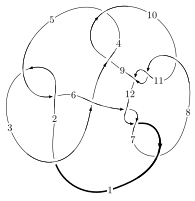
\includegraphics[width=112pt]{../../../GIT/diagram.site/Diagrams/png/837_12a_0036.png}\\
\ \ \ A knot diagram\footnotemark}&
\allowdisplaybreaks
\textbf{Linearized knot diagam} \\
\cline{2-2}
 &
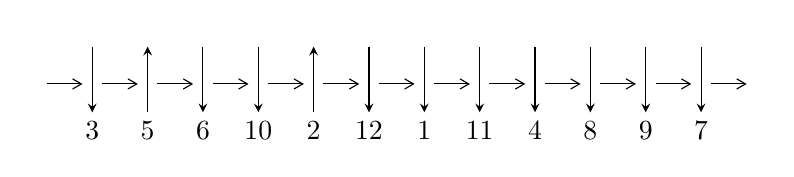
\begin{tikzpicture}[x=20pt, y=17pt]
	% nodes
	\node (C0) at (0, 0) {};
	\node (C1) at (1, 0) {};
	\node (C1U) at (1, +1) {};
	\node (C1D) at (1, -1) {3};

	\node (C2) at (2, 0) {};
	\node (C2U) at (2, +1) {};
	\node (C2D) at (2, -1) {5};

	\node (C3) at (3, 0) {};
	\node (C3U) at (3, +1) {};
	\node (C3D) at (3, -1) {6};

	\node (C4) at (4, 0) {};
	\node (C4U) at (4, +1) {};
	\node (C4D) at (4, -1) {10};

	\node (C5) at (5, 0) {};
	\node (C5U) at (5, +1) {};
	\node (C5D) at (5, -1) {2};

	\node (C6) at (6, 0) {};
	\node (C6U) at (6, +1) {};
	\node (C6D) at (6, -1) {12};

	\node (C7) at (7, 0) {};
	\node (C7U) at (7, +1) {};
	\node (C7D) at (7, -1) {1};

	\node (C8) at (8, 0) {};
	\node (C8U) at (8, +1) {};
	\node (C8D) at (8, -1) {11};

	\node (C9) at (9, 0) {};
	\node (C9U) at (9, +1) {};
	\node (C9D) at (9, -1) {4};

	\node (C10) at (10, 0) {};
	\node (C10U) at (10, +1) {};
	\node (C10D) at (10, -1) {8};

	\node (C11) at (11, 0) {};
	\node (C11U) at (11, +1) {};
	\node (C11D) at (11, -1) {9};

	\node (C12) at (12, 0) {};
	\node (C12U) at (12, +1) {};
	\node (C12D) at (12, -1) {7};
	\node (C13) at (13, 0) {};

	% arrows
	\draw[->,>={angle 60}]
	(C0) edge (C1) (C1) edge (C2) (C2) edge (C3) (C3) edge (C4) (C4) edge (C5) (C5) edge (C6) (C6) edge (C7) (C7) edge (C8) (C8) edge (C9) (C9) edge (C10) (C10) edge (C11) (C11) edge (C12) (C12) edge (C13) ;	\draw[->,>=stealth]
	(C1U) edge (C1D) (C2D) edge (C2U) (C3U) edge (C3D) (C4U) edge (C4D) (C5D) edge (C5U) (C6U) edge (C6D) (C7U) edge (C7D) (C8U) edge (C8D) (C9U) edge (C9D) (C10U) edge (C10D) (C11U) edge (C11D) (C12U) edge (C12D) ;
	\end{tikzpicture} \\
\hhline{~~} \\& 
\textbf{Solving Sequence} \\ \cline{2-2} 
 &
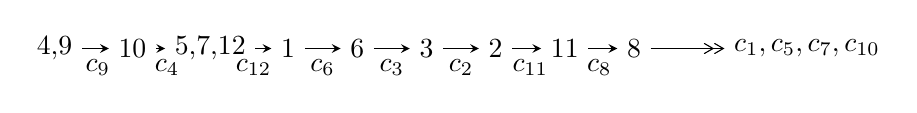
\begin{tikzpicture}[x=25pt, y=7pt]
	% node
	\node (A0) at (-1/8, 0) {4,9};
	\node (A1) at (1, 0) {10};
	\node (A2) at (17/8, 0) {5,7,12};
	\node (A3) at (13/4, 0) {1};
	\node (A4) at (17/4, 0) {6};
	\node (A5) at (21/4, 0) {3};
	\node (A6) at (25/4, 0) {2};
	\node (A7) at (29/4, 0) {11};
	\node (A8) at (33/4, 0) {8};
	\node (C1) at (1/2, -1) {$c_{9}$};
	\node (C2) at (3/2, -1) {$c_{4}$};
	\node (C3) at (11/4, -1) {$c_{12}$};
	\node (C4) at (15/4, -1) {$c_{6}$};
	\node (C5) at (19/4, -1) {$c_{3}$};
	\node (C6) at (23/4, -1) {$c_{2}$};
	\node (C7) at (27/4, -1) {$c_{11}$};
	\node (C8) at (31/4, -1) {$c_{8}$};
	\node (A9) at (43/4, 0) {$c_{1},c_{5},c_{7},c_{10}$};

	% edge
	\draw[->,>=stealth]	
	(A0) edge (A1) (A1) edge (A2) (A2) edge (A3) (A3) edge (A4) (A4) edge (A5) (A5) edge (A6) (A6) edge (A7) (A7) edge (A8) ;
	\draw[->>,>={angle 60}]	
	(A8) edge (A9);
\end{tikzpicture} \\ 

\end{tabular} \\

\footnotetext{
The image of knot diagram is generated by the software ``\textbf{Draw programme}" developed by Andrew Bartholomew(\url{http://www.layer8.co.uk/maths/draw/index.htm\#Running-draw}), where we modified some parts for our purpose(\url{https://github.com/CATsTAILs/LinksPainter}).
}\phantom \\ \newline 
\centering \textbf{Ideals for irreducible components\footnotemark of $X_{\text{par}}$} 
 
\begin{align*}
I^u_{1}&=\langle 
-3.71327\times10^{48} u^{35}+4.04621\times10^{50} u^{34}+\cdots+1.08619\times10^{53} d-2.28969\times10^{52},\\
\phantom{I^u_{1}}&\phantom{= \langle  }5.92442\times10^{49} u^{35}-1.37260\times10^{51} u^{34}+\cdots+2.17237\times10^{53} c-1.61328\times10^{53},\\
\phantom{I^u_{1}}&\phantom{= \langle  }1.56429\times10^{50} u^{35}-1.90035\times10^{51} u^{34}+\cdots+1.08619\times10^{53} b+1.05897\times10^{53},\\
\phantom{I^u_{1}}&\phantom{= \langle  }-1.77635\times10^{50} u^{35}+8.48997\times10^{50} u^{34}+\cdots+1.08619\times10^{53} a-1.56178\times10^{53},\\
\phantom{I^u_{1}}&\phantom{= \langle  }u^{36}-3 u^{35}+\cdots-64 u+32\rangle \\
I^u_{2}&=\langle 
1.13466\times10^{15} a u^{27}-3.06796\times10^{15} u^{27}+\cdots+2.79964\times10^{15} a-1.43321\times10^{16},\\
\phantom{I^u_{2}}&\phantom{= \langle  }-6.13592\times10^{15} a u^{27}-7.57070\times10^{15} u^{27}+\cdots-2.86643\times10^{16} a-2.56902\times10^{16},\;b+1,\\
\phantom{I^u_{2}}&\phantom{= \langle  }2.13254\times10^{15} a u^{27}+1.47729\times10^{16} u^{27}+\cdots+2.93914\times10^{16} a+7.21477\times10^{16},\;u^{28}+u^{27}+\cdots+8 u+4\rangle \\
\\
I^v_{1}&=\langle 
a,\;d,\;c-1,\;b+1,\;v^2+v+1\rangle \\
I^v_{2}&=\langle 
a,\;d-1,\;c+a,\;b+1,\;v^2+v+1\rangle \\
I^v_{3}&=\langle 
a,\;d-1,\;c+a+1,\;b+1,\;v+1\rangle \\
I^v_{4}&=\langle 
c,\;d-1,\;c b- a-1,\;v^2 b a+v^2 c+v^2 b+2 v^2 a+c v+a v+2 v^2+c+v,\;b^2 v^2+2 v^2 b+b v+v^2+v+1\rangle \\
\end{align*}
\raggedright * 5 irreducible components of $\dim_{\mathbb{C}}=0$, with total 97 representations.\\
\raggedright * 1 irreducible components of $\dim_{\mathbb{C}}=1$ \\
\footnotetext{All coefficients of polynomials are rational numbers. But the coefficients are sometimes approximated in decimal forms when there is not enough margin.}
\newpage
\renewcommand{\arraystretch}{1}
\centering \section*{I. $I^u_{1}= \langle -3.71\times10^{48} u^{35}+4.05\times10^{50} u^{34}+\cdots+1.09\times10^{53} d-2.29\times10^{52},\;5.92\times10^{49} u^{35}-1.37\times10^{51} u^{34}+\cdots+2.17\times10^{53} c-1.61\times10^{53},\;1.56\times10^{50} u^{35}-1.90\times10^{51} u^{34}+\cdots+1.09\times10^{53} b+1.06\times10^{53},\;-1.78\times10^{50} u^{35}+8.49\times10^{50} u^{34}+\cdots+1.09\times10^{53} a-1.56\times10^{53},\;u^{36}-3 u^{35}+\cdots-64 u+32 \rangle$}
\flushleft \textbf{(i) Arc colorings}\\
\begin{tabular}{m{7pt} m{180pt} m{7pt} m{180pt} }
\flushright $a_{4}=$&$\begin{pmatrix}0\\u\end{pmatrix}$ \\
\flushright $a_{9}=$&$\begin{pmatrix}1\\0\end{pmatrix}$ \\
\flushright $a_{10}=$&$\begin{pmatrix}1\\u^2\end{pmatrix}$ \\
\flushright $a_{5}=$&$\begin{pmatrix}- u\\- u^3+u\end{pmatrix}$ \\
\flushright $a_{7}=$&$\begin{pmatrix}0.00163541 u^{35}-0.00781632 u^{34}+\cdots-1.02250 u+1.43786\\-0.00144017 u^{35}+0.0174956 u^{34}+\cdots+2.23968 u-0.974944\end{pmatrix}$ \\
\flushright $a_{12}=$&$\begin{pmatrix}-0.000272717 u^{35}+0.00631846 u^{34}+\cdots+0.563935 u+0.742637\\0.0000341864 u^{35}-0.00372516 u^{34}+\cdots-0.444645 u+0.210801\end{pmatrix}$ \\
\flushright $a_{1}=$&$\begin{pmatrix}-0.0000432971 u^{35}+0.0122726 u^{34}+\cdots+1.33646 u+0.416353\\0.00188305 u^{35}-0.0189570 u^{34}+\cdots-2.03361 u+0.857265\end{pmatrix}$ \\
\flushright $a_{6}=$&$\begin{pmatrix}0.000904113 u^{35}-0.00884304 u^{34}+\cdots-1.47566 u+1.66218\\-0.000947410 u^{35}+0.0211156 u^{34}+\cdots+2.81213 u-1.24583\end{pmatrix}$ \\
\flushright $a_{3}=$&$\begin{pmatrix}0.00194611 u^{35}-0.00144413 u^{34}+\cdots+2.53686 u-0.189589\\0.0137165 u^{35}-0.0449480 u^{34}+\cdots-0.634013 u+0.309094\end{pmatrix}$ \\
\flushright $a_{2}=$&$\begin{pmatrix}0.00349030 u^{35}-0.000257565 u^{34}+\cdots+3.44348 u-0.336815\\0.0131839 u^{35}-0.0436398 u^{34}+\cdots-1.21762 u+0.270108\end{pmatrix}$ \\
\flushright $a_{11}=$&$\begin{pmatrix}-0.000238531 u^{35}+0.00259330 u^{34}+\cdots+0.119290 u+0.953438\\0.0000341864 u^{35}-0.00372516 u^{34}+\cdots-0.444645 u+0.210801\end{pmatrix}$ \\
\flushright $a_{8}=$&$\begin{pmatrix}-0.000238531 u^{35}+0.00259330 u^{34}+\cdots+0.119290 u+0.953438\\0.000492763 u^{35}+0.00362002 u^{34}+\cdots+0.572452 u-0.270888\end{pmatrix}$\\&\end{tabular}
\flushleft \textbf{(ii) Obstruction class $= -1$}\\~\\
\flushleft \textbf{(iii) Cusp Shapes $= 0.0805025 u^{35}-0.242112 u^{34}+\cdots+5.72407 u-9.52193$}\\~\\
\newpage\renewcommand{\arraystretch}{1}
\flushleft \textbf{(iv) u-Polynomials at the component}\newline \\
\begin{tabular}{m{50pt}|m{274pt}}
Crossings & \hspace{64pt}u-Polynomials at each crossing \\
\hline $$\begin{aligned}c_{1}\end{aligned}$$&$\begin{aligned}
&u^{36}+17 u^{35}+\cdots-120 u+16
\end{aligned}$\\
\hline $$\begin{aligned}c_{2},c_{5}\end{aligned}$$&$\begin{aligned}
&u^{36}+u^{35}+\cdots+16 u+4
\end{aligned}$\\
\hline $$\begin{aligned}c_{3}\end{aligned}$$&$\begin{aligned}
&u^{36}- u^{35}+\cdots-104 u+1252
\end{aligned}$\\
\hline $$\begin{aligned}c_{4},c_{9}\end{aligned}$$&$\begin{aligned}
&u^{36}+3 u^{35}+\cdots+64 u+32
\end{aligned}$\\
\hline $$\begin{aligned}c_{6},c_{7},c_{8}\\c_{10},c_{11},c_{12}\end{aligned}$$&$\begin{aligned}
&u^{36}-5 u^{35}+\cdots+3 u-1
\end{aligned}$\\
\hline
\end{tabular}\\~\\
\newpage\renewcommand{\arraystretch}{1}
\flushleft \textbf{(v) Riley Polynomials at the component}\newline \\
\begin{tabular}{m{50pt}|m{274pt}}
Crossings & \hspace{64pt}Riley Polynomials at each crossing \\
\hline $$\begin{aligned}c_{1}\end{aligned}$$&$\begin{aligned}
&y^{36}+5 y^{35}+\cdots-27936 y+256
\end{aligned}$\\
\hline $$\begin{aligned}c_{2},c_{5}\end{aligned}$$&$\begin{aligned}
&y^{36}+17 y^{35}+\cdots-120 y+16
\end{aligned}$\\
\hline $$\begin{aligned}c_{3}\end{aligned}$$&$\begin{aligned}
&y^{36}-7 y^{35}+\cdots-22103608 y+1567504
\end{aligned}$\\
\hline $$\begin{aligned}c_{4},c_{9}\end{aligned}$$&$\begin{aligned}
&y^{36}-15 y^{35}+\cdots-1024 y+1024
\end{aligned}$\\
\hline $$\begin{aligned}c_{6},c_{7},c_{8}\\c_{10},c_{11},c_{12}\end{aligned}$$&$\begin{aligned}
&y^{36}-41 y^{35}+\cdots-21 y+1
\end{aligned}$\\
\hline
\end{tabular}\\~\\
\newpage\flushleft \textbf{(vi) Complex Volumes and Cusp Shapes}
$$\begin{array}{c|c|c}  
\text{Solutions to }I^u_{1}& \I (\text{vol} + \sqrt{-1}CS) & \text{Cusp shape}\\
 \hline 
\begin{aligned}
u &= \phantom{-}0.956534 + 0.246505 I \\
a &= -0.0142428 + 0.0350628 I \\
b &= \phantom{-}0.595799 - 0.651291 I \\
c &= \phantom{-}0.141093 - 0.856670 I \\
d &= \phantom{-}0.446161 + 0.609262 I\end{aligned}
 & -2.56616 - 0.65266 I & -13.12638 + 3.31133 I \\ \hline\begin{aligned}
u &= \phantom{-}0.956534 - 0.246505 I \\
a &= -0.0142428 - 0.0350628 I \\
b &= \phantom{-}0.595799 + 0.651291 I \\
c &= \phantom{-}0.141093 + 0.856670 I \\
d &= \phantom{-}0.446161 - 0.609262 I\end{aligned}
 & -2.56616 + 0.65266 I & -13.12638 - 3.31133 I \\ \hline\begin{aligned}
u &= -0.935949 + 0.527292 I \\
a &= -0.118634 + 0.273971 I \\
b &= \phantom{-}0.711040 + 0.301202 I \\
c &= \phantom{-}0.364553 + 1.079240 I \\
d &= \phantom{-}0.236726 - 0.726179 I\end{aligned}
 & \phantom{-}1.36964 + 3.10356 I & -5.16268 - 4.71165 I \\ \hline\begin{aligned}
u &= -0.935949 - 0.527292 I \\
a &= -0.118634 - 0.273971 I \\
b &= \phantom{-}0.711040 - 0.301202 I \\
c &= \phantom{-}0.364553 - 1.079240 I \\
d &= \phantom{-}0.236726 + 0.726179 I\end{aligned}
 & \phantom{-}1.36964 - 3.10356 I & -5.16268 + 4.71165 I \\ \hline\begin{aligned}
u &= -0.651308 + 0.620650 I \\
a &= \phantom{-}0.088381 + 0.613358 I \\
b &= \phantom{-}0.525117 + 0.024485 I \\
c &= \phantom{-}0.711979 + 1.024680 I \\
d &= \phantom{-}0.018859 - 0.596676 I\end{aligned}
 & \phantom{-}2.25394 + 1.43184 I & -2.05632 - 3.52848 I \\ \hline\begin{aligned}
u &= -0.651308 - 0.620650 I \\
a &= \phantom{-}0.088381 - 0.613358 I \\
b &= \phantom{-}0.525117 - 0.024485 I \\
c &= \phantom{-}0.711979 - 1.024680 I \\
d &= \phantom{-}0.018859 + 0.596676 I\end{aligned}
 & \phantom{-}2.25394 - 1.43184 I & -2.05632 + 3.52848 I\\
 \hline 
 \end{array}$$\newpage$$\begin{array}{c|c|c}  
\text{Solutions to }I^u_{1}& \I (\text{vol} + \sqrt{-1}CS) & \text{Cusp shape}\\
 \hline 
\begin{aligned}
u &= -0.134519 + 0.831817 I \\
a &= -2.49461 + 0.46036 I \\
b &= \phantom{-}5.38486 - 0.94232 I \\
c &= -0.800905 - 0.073407 I \\
d &= \phantom{-}1.245840 + 0.061269 I\end{aligned}
 & -4.07214 - 2.53804 I & -12.12047 + 3.16226 I \\ \hline\begin{aligned}
u &= -0.134519 - 0.831817 I \\
a &= -2.49461 - 0.46036 I \\
b &= \phantom{-}5.38486 + 0.94232 I \\
c &= -0.800905 + 0.073407 I \\
d &= \phantom{-}1.245840 - 0.061269 I\end{aligned}
 & -4.07214 + 2.53804 I & -12.12047 - 3.16226 I \\ \hline\begin{aligned}
u &= \phantom{-}0.488093 + 0.675929 I \\
a &= \phantom{-}0.219986 - 0.913847 I \\
b &= \phantom{-}0.439268 + 0.155961 I \\
c &= \phantom{-}0.951048 - 1.034360 I \\
d &= -0.119169 + 0.531960 I\end{aligned}
 & \phantom{-}0.92725 + 3.15352 I & -4.07893 - 3.45921 I \\ \hline\begin{aligned}
u &= \phantom{-}0.488093 - 0.675929 I \\
a &= \phantom{-}0.219986 + 0.913847 I \\
b &= \phantom{-}0.439268 - 0.155961 I \\
c &= \phantom{-}0.951048 + 1.034360 I \\
d &= -0.119169 - 0.531960 I\end{aligned}
 & \phantom{-}0.92725 - 3.15352 I & -4.07893 + 3.45921 I \\ \hline\begin{aligned}
u &= \phantom{-}1.066500 + 0.529753 I \\
a &= -0.230642 - 0.205554 I \\
b &= \phantom{-}0.835462 - 0.357382 I \\
c &= \phantom{-}0.257325 - 1.157650 I \\
d &= \phantom{-}0.296959 + 0.811036 I\end{aligned}
 & -0.85359 - 7.85577 I & -9.34096 + 8.43490 I \\ \hline\begin{aligned}
u &= \phantom{-}1.066500 - 0.529753 I \\
a &= -0.230642 + 0.205554 I \\
b &= \phantom{-}0.835462 + 0.357382 I \\
c &= \phantom{-}0.257325 + 1.157650 I \\
d &= \phantom{-}0.296959 - 0.811036 I\end{aligned}
 & -0.85359 + 7.85577 I & -9.34096 - 8.43490 I\\
 \hline 
 \end{array}$$\newpage$$\begin{array}{c|c|c}  
\text{Solutions to }I^u_{1}& \I (\text{vol} + \sqrt{-1}CS) & \text{Cusp shape}\\
 \hline 
\begin{aligned}
u &= -0.471804 + 1.201650 I \\
a &= -1.55056 + 0.44817 I \\
b &= \phantom{-}3.43387 - 0.95934 I \\
c &= -1.009840 - 0.265513 I \\
d &= \phantom{-}1.41953 + 0.22707 I\end{aligned}
 & -6.92260 - 4.39379 I & -12.55418 + 2.40542 I \\ \hline\begin{aligned}
u &= -0.471804 - 1.201650 I \\
a &= -1.55056 - 0.44817 I \\
b &= \phantom{-}3.43387 + 0.95934 I \\
c &= -1.009840 + 0.265513 I \\
d &= \phantom{-}1.41953 - 0.22707 I\end{aligned}
 & -6.92260 + 4.39379 I & -12.55418 - 2.40542 I \\ \hline\begin{aligned}
u &= \phantom{-}1.232210 + 0.408112 I \\
a &= \phantom{-}1.16290 - 2.88555 I \\
b &= \phantom{-}3.50484 - 0.82980 I \\
c &= -0.478569 + 1.058540 I \\
d &= -1.43441 - 0.19589 I\end{aligned}
 & -8.11992 - 1.67660 I & -15.7568 + 0.9806 I \\ \hline\begin{aligned}
u &= \phantom{-}1.232210 - 0.408112 I \\
a &= \phantom{-}1.16290 + 2.88555 I \\
b &= \phantom{-}3.50484 + 0.82980 I \\
c &= -0.478569 - 1.058540 I \\
d &= -1.43441 + 0.19589 I\end{aligned}
 & -8.11992 + 1.67660 I & -15.7568 - 0.9806 I \\ \hline\begin{aligned}
u &= -1.223950 + 0.516090 I \\
a &= \phantom{-}0.35261 + 3.02077 I \\
b &= \phantom{-}3.33397 + 0.96426 I \\
c &= -0.310513 - 1.254720 I \\
d &= -1.43061 + 0.24878 I\end{aligned}
 & -7.33125 + 7.52384 I & -14.0983 - 6.1679 I \\ \hline\begin{aligned}
u &= -1.223950 - 0.516090 I \\
a &= \phantom{-}0.35261 - 3.02077 I \\
b &= \phantom{-}3.33397 - 0.96426 I \\
c &= -0.310513 + 1.254720 I \\
d &= -1.43061 - 0.24878 I\end{aligned}
 & -7.33125 - 7.52384 I & -14.0983 + 6.1679 I\\
 \hline 
 \end{array}$$\newpage$$\begin{array}{c|c|c}  
\text{Solutions to }I^u_{1}& \I (\text{vol} + \sqrt{-1}CS) & \text{Cusp shape}\\
 \hline 
\begin{aligned}
u &= -0.666134 + 0.068993 I \\
a &= \phantom{-}0.780189 + 0.682100 I \\
b &= -0.90161 - 1.52116 I \\
c &= -0.128853 - 0.268419 I \\
d &= \phantom{-}0.706776 + 0.200522 I\end{aligned}
 & -2.77509 - 2.72721 I & -16.6085 + 5.9652 I \\ \hline\begin{aligned}
u &= -0.666134 - 0.068993 I \\
a &= \phantom{-}0.780189 - 0.682100 I \\
b &= -0.90161 + 1.52116 I \\
c &= -0.128853 + 0.268419 I \\
d &= \phantom{-}0.706776 - 0.200522 I\end{aligned}
 & -2.77509 + 2.72721 I & -16.6085 - 5.9652 I \\ \hline\begin{aligned}
u &= \phantom{-}0.318666 + 1.335800 I \\
a &= -1.57860 - 0.26349 I \\
b &= \phantom{-}3.47760 + 0.56643 I \\
c &= -1.083360 + 0.176981 I \\
d &= \phantom{-}1.48437 - 0.15238 I\end{aligned}
 & -11.42670 + 0.95860 I & -17.6650 + 0.2050 I \\ \hline\begin{aligned}
u &= \phantom{-}0.318666 - 1.335800 I \\
a &= -1.57860 + 0.26349 I \\
b &= \phantom{-}3.47760 - 0.56643 I \\
c &= -1.083360 - 0.176981 I \\
d &= \phantom{-}1.48437 + 0.15238 I\end{aligned}
 & -11.42670 - 0.95860 I & -17.6650 - 0.2050 I \\ \hline\begin{aligned}
u &= \phantom{-}0.568640 + 1.285090 I \\
a &= -1.44127 - 0.41824 I \\
b &= \phantom{-}3.20069 + 0.90828 I \\
c &= -1.059710 + 0.318993 I \\
d &= \phantom{-}1.46105 - 0.27427 I\end{aligned}
 & -9.63713 + 9.42250 I & -15.4804 - 5.9490 I \\ \hline\begin{aligned}
u &= \phantom{-}0.568640 - 1.285090 I \\
a &= -1.44127 + 0.41824 I \\
b &= \phantom{-}3.20069 - 0.90828 I \\
c &= -1.059710 - 0.318993 I \\
d &= \phantom{-}1.46105 + 0.27427 I\end{aligned}
 & -9.63713 - 9.42250 I & -15.4804 + 5.9490 I\\
 \hline 
 \end{array}$$\newpage$$\begin{array}{c|c|c}  
\text{Solutions to }I^u_{1}& \I (\text{vol} + \sqrt{-1}CS) & \text{Cusp shape}\\
 \hline 
\begin{aligned}
u &= \phantom{-}0.579877\phantom{ +0.000000I} \\
a &= \phantom{-}0.700882\phantom{ +0.000000I} \\
b &= -0.382079\phantom{ +0.000000I} \\
c &= \phantom{-}0.313536\phantom{ +0.000000I} \\
d &= \phantom{-}0.400496\phantom{ +0.000000I}\end{aligned}
 & -0.811618\phantom{ +0.000000I} & -12.0290\phantom{ +0.000000I} \\ \hline\begin{aligned}
u &= -1.27702 + 0.74720 I \\
a &= -0.79571 + 2.33781 I \\
b &= \phantom{-}2.94232 + 0.99996 I \\
c &= \phantom{-}0.11920 - 1.42161 I \\
d &= -1.45945 + 0.36293 I\end{aligned}
 & -9.5381 + 11.3478 I & -13.0594 - 5.6672 I \\ \hline\begin{aligned}
u &= -1.27702 - 0.74720 I \\
a &= -0.79571 - 2.33781 I \\
b &= \phantom{-}2.94232 - 0.99996 I \\
c &= \phantom{-}0.11920 + 1.42161 I \\
d &= -1.45945 - 0.36293 I\end{aligned}
 & -9.5381 - 11.3478 I & -13.0594 + 5.6672 I \\ \hline\begin{aligned}
u &= \phantom{-}1.51924\phantom{ +0.000000I} \\
a &= \phantom{-}1.38331\phantom{ +0.000000I} \\
b &= \phantom{-}3.36154\phantom{ +0.000000I} \\
c &= -0.179172\phantom{ +0.000000I} \\
d &= -1.57128\phantom{ +0.000000I}\end{aligned}
 & -14.8609\phantom{ +0.000000I} & -15.8600\phantom{ +0.000000I} \\ \hline\begin{aligned}
u &= \phantom{-}1.29117 + 0.81558 I \\
a &= -0.98989 - 2.12524 I \\
b &= \phantom{-}2.84808 - 0.99055 I \\
c &= \phantom{-}0.22492 + 1.45088 I \\
d &= -1.46798 - 0.39682 I\end{aligned}
 & -12.0349 - 16.8809 I & -15.3736 + 9.2575 I \\ \hline\begin{aligned}
u &= \phantom{-}1.29117 - 0.81558 I \\
a &= -0.98989 + 2.12524 I \\
b &= \phantom{-}2.84808 + 0.99055 I \\
c &= \phantom{-}0.22492 - 1.45088 I \\
d &= -1.46798 + 0.39682 I\end{aligned}
 & -12.0349 + 16.8809 I & -15.3736 - 9.2575 I\\
 \hline 
 \end{array}$$\newpage$$\begin{array}{c|c|c}  
\text{Solutions to }I^u_{1}& \I (\text{vol} + \sqrt{-1}CS) & \text{Cusp shape}\\
 \hline 
\begin{aligned}
u &= \phantom{-}0.111921 + 0.451208 I \\
a &= \phantom{-}1.46514 - 0.45120 I \\
b &= -0.0451061 + 0.0894307 I \\
c &= \phantom{-}1.40357 - 0.27941 I \\
d &= -0.190856 + 0.111820 I\end{aligned}
 & -0.30692 - 1.79670 I & -2.13838 + 3.34715 I \\ \hline\begin{aligned}
u &= \phantom{-}0.111921 - 0.451208 I \\
a &= \phantom{-}1.46514 + 0.45120 I \\
b &= -0.0451061 - 0.0894307 I \\
c &= \phantom{-}1.40357 + 0.27941 I \\
d &= -0.190856 - 0.111820 I\end{aligned}
 & -0.30692 + 1.79670 I & -2.13838 - 3.34715 I \\ \hline\begin{aligned}
u &= \phantom{-}1.38860 + 0.67758 I \\
a &= -0.35175 - 2.03094 I \\
b &= \phantom{-}2.99578 - 0.83109 I \\
c &= \phantom{-}0.126360 + 1.208340 I \\
d &= -1.51341 - 0.32643 I\end{aligned}
 & -15.0030 - 8.0885 I & -18.3300 + 3.8436 I \\ \hline\begin{aligned}
u &= \phantom{-}1.38860 - 0.67758 I \\
a &= -0.35175 + 2.03094 I \\
b &= \phantom{-}2.99578 + 0.83109 I \\
c &= \phantom{-}0.126360 - 1.208340 I \\
d &= -1.51341 + 0.32643 I\end{aligned}
 & -15.0030 + 8.0885 I & -18.3300 - 3.8436 I \\ \hline\begin{aligned}
u &= -1.61122 + 0.12770 I \\
a &= \phantom{-}0.954593 + 0.434273 I \\
b &= \phantom{-}3.22829 + 0.14916 I \\
c &= \phantom{-}0.004513 - 0.218310 I \\
d &= -1.61501 + 0.06033 I\end{aligned}
 & -18.8051 + 4.7571 I & -19.1049 - 3.2273 I \\ \hline\begin{aligned}
u &= -1.61122 - 0.12770 I \\
a &= \phantom{-}0.954593 - 0.434273 I \\
b &= \phantom{-}3.22829 - 0.14916 I \\
c &= \phantom{-}0.004513 + 0.218310 I \\
d &= -1.61501 - 0.06033 I\end{aligned}
 & -18.8051 - 4.7571 I & -19.1049 + 3.2273 I\\
 \hline 
 \end{array}$$\newpage\newpage\renewcommand{\arraystretch}{1}
\centering \section*{II. $I^u_{2}= \langle 1.13\times10^{15} a u^{27}-3.07\times10^{15} u^{27}+\cdots+2.80\times10^{15} a-1.43\times10^{16},\;-6.14\times10^{15} a u^{27}-7.57\times10^{15} u^{27}+\cdots-2.87\times10^{16} a-2.57\times10^{16},\;b+1,\;2.13\times10^{15} a u^{27}+1.48\times10^{16} u^{27}+\cdots+2.94\times10^{16} a+7.21\times10^{16},\;u^{28}+u^{27}+\cdots+8 u+4 \rangle$}
\flushleft \textbf{(i) Arc colorings}\\
\begin{tabular}{m{7pt} m{180pt} m{7pt} m{180pt} }
\flushright $a_{4}=$&$\begin{pmatrix}0\\u\end{pmatrix}$ \\
\flushright $a_{9}=$&$\begin{pmatrix}1\\0\end{pmatrix}$ \\
\flushright $a_{10}=$&$\begin{pmatrix}1\\u^2\end{pmatrix}$ \\
\flushright $a_{5}=$&$\begin{pmatrix}- u\\- u^3+u\end{pmatrix}$ \\
\flushright $a_{7}=$&$\begin{pmatrix}a\\-1\end{pmatrix}$ \\
\flushright $a_{12}=$&$\begin{pmatrix}2.97137 a u^{27}+3.66617 u^{27}+\cdots+13.8809 a+12.4407\\-1.09893 a u^{27}+2.97137 u^{27}+\cdots-2.71150 a+13.8809\end{pmatrix}$ \\
\flushright $a_{1}=$&$\begin{pmatrix}-1.87244 u^{27}-0.749749 u^{26}+\cdots-7.03105 u-11.1694\\1.09893 u^{27}-0.185171 u^{26}+\cdots+5.48839 u+2.71150\end{pmatrix}$ \\
\flushright $a_{6}=$&$\begin{pmatrix}-0.333289 u^{27}-0.505230 u^{26}+\cdots-0.0509032 u-3.96717\\-1.53915 u^{27}-0.244519 u^{26}+\cdots-6.98014 u-7.20224\end{pmatrix}$ \\
\flushright $a_{3}=$&$\begin{pmatrix}-3.54326 u^{27}-0.280326 u^{26}+\cdots-16.6119 u-14.7552\\0.187465 u^{27}-0.126714 u^{26}+\cdots+1.72320 u+0.0904714\end{pmatrix}$ \\
\flushright $a_{2}=$&$\begin{pmatrix}-2.49289 u^{27}-0.296873 u^{26}+\cdots-11.3968 u-10.5619\\0.0560178 u^{27}-0.0365360 u^{26}+\cdots+0.841877 u+0.164880\end{pmatrix}$ \\
\flushright $a_{11}=$&$\begin{pmatrix}1.87244 a u^{27}+6.63754 u^{27}+\cdots+11.1694 a+26.3216\\-1.09893 a u^{27}+2.97137 u^{27}+\cdots-2.71150 a+13.8809\end{pmatrix}$ \\
\flushright $a_{8}=$&$\begin{pmatrix}1.87244 a u^{27}+6.63754 u^{27}+\cdots+11.1694 a+26.3216\\1.53915 a u^{27}+1.87244 u^{27}+\cdots+7.20224 a+9.16941\end{pmatrix}$\\&\end{tabular}
\flushleft \textbf{(ii) Obstruction class $= -1$}\\~\\
\flushleft \textbf{(iii) Cusp Shapes $= \frac{37274533074785}{129063433504426} u^{27}+\frac{53621307092165}{129063433504426} u^{26}+\cdots+\frac{660629047616669}{129063433504426} u-\frac{645502044434670}{64531716752213}$}\\~\\
\newpage\renewcommand{\arraystretch}{1}
\flushleft \textbf{(iv) u-Polynomials at the component}\newline \\
\begin{tabular}{m{50pt}|m{274pt}}
Crossings & \hspace{64pt}u-Polynomials at each crossing \\
\hline $$\begin{aligned}c_{1}\end{aligned}$$&$\begin{aligned}
&(u^{28}+14 u^{27}+\cdots+2 u+1)^{2}
\end{aligned}$\\
\hline $$\begin{aligned}c_{2},c_{5}\end{aligned}$$&$\begin{aligned}
&(u^{28}+2 u^{27}+\cdots+2 u+1)^{2}
\end{aligned}$\\
\hline $$\begin{aligned}c_{3}\end{aligned}$$&$\begin{aligned}
&(u^{28}-2 u^{27}+\cdots-22 u+17)^{2}
\end{aligned}$\\
\hline $$\begin{aligned}c_{4},c_{9}\end{aligned}$$&$\begin{aligned}
&(u^{28}- u^{27}+\cdots-8 u+4)^{2}
\end{aligned}$\\
\hline $$\begin{aligned}c_{6},c_{7},c_{8}\\c_{10},c_{11},c_{12}\end{aligned}$$&$\begin{aligned}
&u^{56}-3 u^{55}+\cdots+72 u+16
\end{aligned}$\\
\hline
\end{tabular}\\~\\
\newpage\renewcommand{\arraystretch}{1}
\flushleft \textbf{(v) Riley Polynomials at the component}\newline \\
\begin{tabular}{m{50pt}|m{274pt}}
Crossings & \hspace{64pt}Riley Polynomials at each crossing \\
\hline $$\begin{aligned}c_{1}\end{aligned}$$&$\begin{aligned}
&(y^{28}+2 y^{27}+\cdots+14 y+1)^{2}
\end{aligned}$\\
\hline $$\begin{aligned}c_{2},c_{5}\end{aligned}$$&$\begin{aligned}
&(y^{28}+14 y^{27}+\cdots+2 y+1)^{2}
\end{aligned}$\\
\hline $$\begin{aligned}c_{3}\end{aligned}$$&$\begin{aligned}
&(y^{28}-10 y^{27}+\cdots-246 y+289)^{2}
\end{aligned}$\\
\hline $$\begin{aligned}c_{4},c_{9}\end{aligned}$$&$\begin{aligned}
&(y^{28}-15 y^{27}+\cdots-88 y+16)^{2}
\end{aligned}$\\
\hline $$\begin{aligned}c_{6},c_{7},c_{8}\\c_{10},c_{11},c_{12}\end{aligned}$$&$\begin{aligned}
&y^{56}-43 y^{55}+\cdots+736 y+256
\end{aligned}$\\
\hline
\end{tabular}\\~\\
\newpage\flushleft \textbf{(vi) Complex Volumes and Cusp Shapes}
$$\begin{array}{c|c|c}  
\text{Solutions to }I^u_{2}& \I (\text{vol} + \sqrt{-1}CS) & \text{Cusp shape}\\
 \hline 
\begin{aligned}
u &= \phantom{-}0.910131 + 0.395689 I \\
a &= -1.02788 + 1.10315 I \\
b &= -1.00000\phantom{ +0.000000I} \\
c &= -1.20522 + 1.86019 I \\
d &= -1.276980 - 0.186733 I\end{aligned}
 & -1.72215 - 4.24816 I & -10.11355 + 6.97904 I \\ \hline\begin{aligned}
u &= \phantom{-}0.910131 + 0.395689 I \\
a &= -0.01361 + 2.44534 I \\
b &= -1.00000\phantom{ +0.000000I} \\
c &= \phantom{-}0.300677 - 0.944242 I \\
d &= \phantom{-}0.313357 + 0.643423 I\end{aligned}
 & -1.72215 - 4.24816 I & -10.11355 + 6.97904 I \\ \hline\begin{aligned}
u &= \phantom{-}0.910131 - 0.395689 I \\
a &= -1.02788 - 1.10315 I \\
b &= -1.00000\phantom{ +0.000000I} \\
c &= -1.20522 - 1.86019 I \\
d &= -1.276980 + 0.186733 I\end{aligned}
 & -1.72215 + 4.24816 I & -10.11355 - 6.97904 I \\ \hline\begin{aligned}
u &= \phantom{-}0.910131 - 0.395689 I \\
a &= -0.01361 - 2.44534 I \\
b &= -1.00000\phantom{ +0.000000I} \\
c &= \phantom{-}0.300677 + 0.944242 I \\
d &= \phantom{-}0.313357 - 0.643423 I\end{aligned}
 & -1.72215 + 4.24816 I & -10.11355 - 6.97904 I \\ \hline\begin{aligned}
u &= -0.017123 + 0.961380 I \\
a &= \phantom{-}0.177063 - 0.402321 I \\
b &= -1.00000\phantom{ +0.000000I} \\
c &= -0.873117 - 0.009489 I \\
d &= \phantom{-}1.306640 + 0.007988 I\end{aligned}
 & -4.61196 + 1.34593 I & -13.91932 - 0.66126 I \\ \hline\begin{aligned}
u &= -0.017123 + 0.961380 I \\
a &= \phantom{-}1.58097 + 1.51341 I \\
b &= -1.00000\phantom{ +0.000000I} \\
c &= \phantom{-}1.50836 + 1.81823 I \\
d &= -0.638546 - 0.533764 I\end{aligned}
 & -4.61196 + 1.34593 I & -13.91932 - 0.66126 I\\
 \hline 
 \end{array}$$\newpage$$\begin{array}{c|c|c}  
\text{Solutions to }I^u_{2}& \I (\text{vol} + \sqrt{-1}CS) & \text{Cusp shape}\\
 \hline 
\begin{aligned}
u &= -0.017123 - 0.961380 I \\
a &= \phantom{-}0.177063 + 0.402321 I \\
b &= -1.00000\phantom{ +0.000000I} \\
c &= -0.873117 + 0.009489 I \\
d &= \phantom{-}1.306640 - 0.007988 I\end{aligned}
 & -4.61196 - 1.34593 I & -13.91932 + 0.66126 I \\ \hline\begin{aligned}
u &= -0.017123 - 0.961380 I \\
a &= \phantom{-}1.58097 - 1.51341 I \\
b &= -1.00000\phantom{ +0.000000I} \\
c &= \phantom{-}1.50836 - 1.81823 I \\
d &= -0.638546 + 0.533764 I\end{aligned}
 & -4.61196 - 1.34593 I & -13.91932 + 0.66126 I \\ \hline\begin{aligned}
u &= -0.907099 + 0.252760 I \\
a &= \phantom{-}0.971495 + 0.463170 I \\
b &= -1.00000\phantom{ +0.000000I} \\
c &= \phantom{-}0.186210 + 0.817511 I \\
d &= \phantom{-}0.419544 - 0.572998 I\end{aligned}
 & -2.63794 + 3.28147 I & -13.2327 - 4.9939 I \\ \hline\begin{aligned}
u &= -0.907099 + 0.252760 I \\
a &= \phantom{-}0.704043 - 0.365524 I \\
b &= -1.00000\phantom{ +0.000000I} \\
c &= -0.351737 - 0.579401 I \\
d &= \phantom{-}0.859190 + 0.455166 I\end{aligned}
 & -2.63794 + 3.28147 I & -13.2327 - 4.9939 I \\ \hline\begin{aligned}
u &= -0.907099 - 0.252760 I \\
a &= \phantom{-}0.971495 - 0.463170 I \\
b &= -1.00000\phantom{ +0.000000I} \\
c &= \phantom{-}0.186210 - 0.817511 I \\
d &= \phantom{-}0.419544 + 0.572998 I\end{aligned}
 & -2.63794 - 3.28147 I & -13.2327 + 4.9939 I \\ \hline\begin{aligned}
u &= -0.907099 - 0.252760 I \\
a &= \phantom{-}0.704043 + 0.365524 I \\
b &= -1.00000\phantom{ +0.000000I} \\
c &= -0.351737 + 0.579401 I \\
d &= \phantom{-}0.859190 - 0.455166 I\end{aligned}
 & -2.63794 - 3.28147 I & -13.2327 + 4.9939 I\\
 \hline 
 \end{array}$$\newpage$$\begin{array}{c|c|c}  
\text{Solutions to }I^u_{2}& \I (\text{vol} + \sqrt{-1}CS) & \text{Cusp shape}\\
 \hline 
\begin{aligned}
u &= \phantom{-}0.387411 + 0.832689 I \\
a &= \phantom{-}0.365520 + 0.349527 I \\
b &= -1.00000\phantom{ +0.000000I} \\
c &= -0.795695 + 0.216194 I \\
d &= \phantom{-}1.239370 - 0.180444 I\end{aligned}
 & -1.43770 + 1.40144 I & -7.30053 - 1.74630 I \\ \hline\begin{aligned}
u &= \phantom{-}0.387411 + 0.832689 I \\
a &= \phantom{-}1.42688 - 0.89203 I \\
b &= -1.00000\phantom{ +0.000000I} \\
c &= \phantom{-}1.11790 - 1.26235 I \\
d &= -0.279611 + 0.583432 I\end{aligned}
 & -1.43770 + 1.40144 I & -7.30053 - 1.74630 I \\ \hline\begin{aligned}
u &= \phantom{-}0.387411 - 0.832689 I \\
a &= \phantom{-}0.365520 - 0.349527 I \\
b &= -1.00000\phantom{ +0.000000I} \\
c &= -0.795695 - 0.216194 I \\
d &= \phantom{-}1.239370 + 0.180444 I\end{aligned}
 & -1.43770 - 1.40144 I & -7.30053 + 1.74630 I \\ \hline\begin{aligned}
u &= \phantom{-}0.387411 - 0.832689 I \\
a &= \phantom{-}1.42688 + 0.89203 I \\
b &= -1.00000\phantom{ +0.000000I} \\
c &= \phantom{-}1.11790 + 1.26235 I \\
d &= -0.279611 - 0.583432 I\end{aligned}
 & -1.43770 - 1.40144 I & -7.30053 + 1.74630 I \\ \hline\begin{aligned}
u &= -0.387502 + 1.047530 I \\
a &= \phantom{-}0.340954 - 0.431763 I \\
b &= -1.00000\phantom{ +0.000000I} \\
c &= -0.920428 - 0.218491 I \\
d &= \phantom{-}1.344350 + 0.185032 I\end{aligned}
 & -3.70255 - 5.75423 I & -11.89302 + 5.96655 I \\ \hline\begin{aligned}
u &= -0.387502 + 1.047530 I \\
a &= \phantom{-}1.27979 + 1.06278 I \\
b &= -1.00000\phantom{ +0.000000I} \\
c &= \phantom{-}1.05142 + 1.53293 I \\
d &= -0.382179 - 0.735842 I\end{aligned}
 & -3.70255 - 5.75423 I & -11.89302 + 5.96655 I\\
 \hline 
 \end{array}$$\newpage$$\begin{array}{c|c|c}  
\text{Solutions to }I^u_{2}& \I (\text{vol} + \sqrt{-1}CS) & \text{Cusp shape}\\
 \hline 
\begin{aligned}
u &= -0.387502 - 1.047530 I \\
a &= \phantom{-}0.340954 + 0.431763 I \\
b &= -1.00000\phantom{ +0.000000I} \\
c &= -0.920428 + 0.218491 I \\
d &= \phantom{-}1.344350 - 0.185032 I\end{aligned}
 & -3.70255 + 5.75423 I & -11.89302 - 5.96655 I \\ \hline\begin{aligned}
u &= -0.387502 - 1.047530 I \\
a &= \phantom{-}1.27979 - 1.06278 I \\
b &= -1.00000\phantom{ +0.000000I} \\
c &= \phantom{-}1.05142 - 1.53293 I \\
d &= -0.382179 + 0.735842 I\end{aligned}
 & -3.70255 + 5.75423 I & -11.89302 - 5.96655 I \\ \hline\begin{aligned}
u &= -0.802767 + 0.244916 I \\
a &= -2.05210 - 1.27314 I \\
b &= -1.00000\phantom{ +0.000000I} \\
c &= -2.29143 - 1.82037 I \\
d &= -1.229860 + 0.111546 I\end{aligned}
 & -2.32218 - 0.90628 I & -12.59768 - 1.67094 I \\ \hline\begin{aligned}
u &= -0.802767 + 0.244916 I \\
a &= -0.72932 - 2.54382 I \\
b &= -1.00000\phantom{ +0.000000I} \\
c &= \phantom{-}0.273098 + 0.711267 I \\
d &= \phantom{-}0.374376 - 0.483492 I\end{aligned}
 & -2.32218 - 0.90628 I & -12.59768 - 1.67094 I \\ \hline\begin{aligned}
u &= -0.802767 - 0.244916 I \\
a &= -2.05210 + 1.27314 I \\
b &= -1.00000\phantom{ +0.000000I} \\
c &= -2.29143 + 1.82037 I \\
d &= -1.229860 - 0.111546 I\end{aligned}
 & -2.32218 + 0.90628 I & -12.59768 + 1.67094 I \\ \hline\begin{aligned}
u &= -0.802767 - 0.244916 I \\
a &= -0.72932 + 2.54382 I \\
b &= -1.00000\phantom{ +0.000000I} \\
c &= \phantom{-}0.273098 - 0.711267 I \\
d &= \phantom{-}0.374376 + 0.483492 I\end{aligned}
 & -2.32218 + 0.90628 I & -12.59768 + 1.67094 I\\
 \hline 
 \end{array}$$\newpage$$\begin{array}{c|c|c}  
\text{Solutions to }I^u_{2}& \I (\text{vol} + \sqrt{-1}CS) & \text{Cusp shape}\\
 \hline 
\begin{aligned}
u &= -1.147340 + 0.340892 I \\
a &= -0.224291 + 1.144170 I \\
b &= -1.00000\phantom{ +0.000000I} \\
c &= -0.471254 - 0.771751 I \\
d &= \phantom{-}0.938913 + 0.621780 I\end{aligned}
 & -5.81300 + 1.47542 I & -13.29345 - 0.59666 I \\ \hline\begin{aligned}
u &= -1.147340 + 0.340892 I \\
a &= -1.07497 - 1.33487 I \\
b &= -1.00000\phantom{ +0.000000I} \\
c &= -0.776477 - 1.062760 I \\
d &= -1.393270 + 0.163069 I\end{aligned}
 & -5.81300 + 1.47542 I & -13.29345 - 0.59666 I \\ \hline\begin{aligned}
u &= -1.147340 - 0.340892 I \\
a &= -0.224291 - 1.144170 I \\
b &= -1.00000\phantom{ +0.000000I} \\
c &= -0.471254 + 0.771751 I \\
d &= \phantom{-}0.938913 - 0.621780 I\end{aligned}
 & -5.81300 - 1.47542 I & -13.29345 + 0.59666 I \\ \hline\begin{aligned}
u &= -1.147340 - 0.340892 I \\
a &= -1.07497 + 1.33487 I \\
b &= -1.00000\phantom{ +0.000000I} \\
c &= -0.776477 + 1.062760 I \\
d &= -1.393270 - 0.163069 I\end{aligned}
 & -5.81300 - 1.47542 I & -13.29345 + 0.59666 I \\ \hline\begin{aligned}
u &= \phantom{-}0.611767 + 0.458091 I \\
a &= \phantom{-}1.235620 - 0.499323 I \\
b &= -1.00000\phantom{ +0.000000I} \\
c &= \phantom{-}0.669435 - 0.799308 I \\
d &= \phantom{-}0.099411 + 0.470368 I\end{aligned}
 & -0.887541 + 0.644142 I & -7.64602 + 1.30683 I \\ \hline\begin{aligned}
u &= \phantom{-}0.611767 + 0.458091 I \\
a &= \phantom{-}0.552061 + 0.278825 I \\
b &= -1.00000\phantom{ +0.000000I} \\
c &= -0.542285 + 0.331792 I \\
d &= \phantom{-}1.027130 - 0.267751 I\end{aligned}
 & -0.887541 + 0.644142 I & -7.64602 + 1.30683 I\\
 \hline 
 \end{array}$$\newpage$$\begin{array}{c|c|c}  
\text{Solutions to }I^u_{2}& \I (\text{vol} + \sqrt{-1}CS) & \text{Cusp shape}\\
 \hline 
\begin{aligned}
u &= \phantom{-}0.611767 - 0.458091 I \\
a &= \phantom{-}1.235620 + 0.499323 I \\
b &= -1.00000\phantom{ +0.000000I} \\
c &= \phantom{-}0.669435 + 0.799308 I \\
d &= \phantom{-}0.099411 - 0.470368 I\end{aligned}
 & -0.887541 - 0.644142 I & -7.64602 - 1.30683 I \\ \hline\begin{aligned}
u &= \phantom{-}0.611767 - 0.458091 I \\
a &= \phantom{-}0.552061 - 0.278825 I \\
b &= -1.00000\phantom{ +0.000000I} \\
c &= -0.542285 - 0.331792 I \\
d &= \phantom{-}1.027130 + 0.267751 I\end{aligned}
 & -0.887541 - 0.644142 I & -7.64602 - 1.30683 I \\ \hline\begin{aligned}
u &= \phantom{-}1.175470 + 0.589984 I \\
a &= -0.299231 + 0.442331 I \\
b &= -1.00000\phantom{ +0.000000I} \\
c &= -0.23958 + 1.44120 I \\
d &= -1.40691 - 0.28559 I\end{aligned}
 & -3.88965 - 6.77427 I & -10.22594 + 4.95962 I \\ \hline\begin{aligned}
u &= \phantom{-}1.175470 + 0.589984 I \\
a &= \phantom{-}0.42258 + 1.93124 I \\
b &= -1.00000\phantom{ +0.000000I} \\
c &= \phantom{-}0.209555 - 1.262070 I \\
d &= \phantom{-}0.307742 + 0.904345 I\end{aligned}
 & -3.88965 - 6.77427 I & -10.22594 + 4.95962 I \\ \hline\begin{aligned}
u &= \phantom{-}1.175470 - 0.589984 I \\
a &= -0.299231 - 0.442331 I \\
b &= -1.00000\phantom{ +0.000000I} \\
c &= -0.23958 - 1.44120 I \\
d &= -1.40691 + 0.28559 I\end{aligned}
 & -3.88965 + 6.77427 I & -10.22594 - 4.95962 I \\ \hline\begin{aligned}
u &= \phantom{-}1.175470 - 0.589984 I \\
a &= \phantom{-}0.42258 - 1.93124 I \\
b &= -1.00000\phantom{ +0.000000I} \\
c &= \phantom{-}0.209555 + 1.262070 I \\
d &= \phantom{-}0.307742 - 0.904345 I\end{aligned}
 & -3.88965 + 6.77427 I & -10.22594 - 4.95962 I\\
 \hline 
 \end{array}$$\newpage$$\begin{array}{c|c|c}  
\text{Solutions to }I^u_{2}& \I (\text{vol} + \sqrt{-1}CS) & \text{Cusp shape}\\
 \hline 
\begin{aligned}
u &= \phantom{-}1.312590 + 0.177484 I \\
a &= -0.920187 + 0.871890 I \\
b &= -1.00000\phantom{ +0.000000I} \\
c &= -0.575440 + 0.451407 I \\
d &= -1.47301 - 0.08468 I\end{aligned}
 & -9.90219 + 2.08114 I & -17.7960 - 2.7886 I \\ \hline\begin{aligned}
u &= \phantom{-}1.312590 + 0.177484 I \\
a &= -0.113586 - 1.304510 I \\
b &= -1.00000\phantom{ +0.000000I} \\
c &= -0.391157 + 0.943404 I \\
d &= \phantom{-}0.853841 - 0.754977 I\end{aligned}
 & -9.90219 + 2.08114 I & -17.7960 - 2.7886 I \\ \hline\begin{aligned}
u &= \phantom{-}1.312590 - 0.177484 I \\
a &= -0.920187 - 0.871890 I \\
b &= -1.00000\phantom{ +0.000000I} \\
c &= -0.575440 - 0.451407 I \\
d &= -1.47301 + 0.08468 I\end{aligned}
 & -9.90219 - 2.08114 I & -17.7960 + 2.7886 I \\ \hline\begin{aligned}
u &= \phantom{-}1.312590 - 0.177484 I \\
a &= -0.113586 + 1.304510 I \\
b &= -1.00000\phantom{ +0.000000I} \\
c &= -0.391157 - 0.943404 I \\
d &= \phantom{-}0.853841 + 0.754977 I\end{aligned}
 & -9.90219 - 2.08114 I & -17.7960 + 2.7886 I \\ \hline\begin{aligned}
u &= \phantom{-}1.262900 + 0.460239 I \\
a &= -0.110303 - 1.099220 I \\
b &= -1.00000\phantom{ +0.000000I} \\
c &= -0.584732 + 0.832898 I \\
d &= \phantom{-}1.027590 - 0.683591 I\end{aligned}
 & -8.61088 - 6.23266 I & -16.1498 + 4.3008 I \\ \hline\begin{aligned}
u &= \phantom{-}1.262900 + 0.460239 I \\
a &= -0.73910 + 1.34519 I \\
b &= -1.00000\phantom{ +0.000000I} \\
c &= -0.341352 + 1.102730 I \\
d &= -1.44949 - 0.22125 I\end{aligned}
 & -8.61088 - 6.23266 I & -16.1498 + 4.3008 I\\
 \hline 
 \end{array}$$\newpage$$\begin{array}{c|c|c}  
\text{Solutions to }I^u_{2}& \I (\text{vol} + \sqrt{-1}CS) & \text{Cusp shape}\\
 \hline 
\begin{aligned}
u &= \phantom{-}1.262900 - 0.460239 I \\
a &= -0.110303 + 1.099220 I \\
b &= -1.00000\phantom{ +0.000000I} \\
c &= -0.584732 - 0.832898 I \\
d &= \phantom{-}1.027590 + 0.683591 I\end{aligned}
 & -8.61088 + 6.23266 I & -16.1498 - 4.3008 I \\ \hline\begin{aligned}
u &= \phantom{-}1.262900 - 0.460239 I \\
a &= -0.73910 - 1.34519 I \\
b &= -1.00000\phantom{ +0.000000I} \\
c &= -0.341352 - 1.102730 I \\
d &= -1.44949 + 0.22125 I\end{aligned}
 & -8.61088 + 6.23266 I & -16.1498 - 4.3008 I \\ \hline\begin{aligned}
u &= -1.280370 + 0.446560 I \\
a &= -0.502612 - 0.171924 I \\
b &= -1.00000\phantom{ +0.000000I} \\
c &= -0.332736 - 1.053240 I \\
d &= -1.45797 + 0.21451 I\end{aligned}
 & -8.68474 + 3.62399 I & -16.2087 - 2.7619 I \\ \hline\begin{aligned}
u &= -1.280370 + 0.446560 I \\
a &= \phantom{-}0.25189 - 1.78789 I \\
b &= -1.00000\phantom{ +0.000000I} \\
c &= \phantom{-}0.059654 + 1.225020 I \\
d &= \phantom{-}0.436936 - 0.910395 I\end{aligned}
 & -8.68474 + 3.62399 I & -16.2087 - 2.7619 I \\ \hline\begin{aligned}
u &= -1.280370 - 0.446560 I \\
a &= -0.502612 + 0.171924 I \\
b &= -1.00000\phantom{ +0.000000I} \\
c &= -0.332736 + 1.053240 I \\
d &= -1.45797 - 0.21451 I\end{aligned}
 & -8.68474 - 3.62399 I & -16.2087 + 2.7619 I \\ \hline\begin{aligned}
u &= -1.280370 - 0.446560 I \\
a &= \phantom{-}0.25189 + 1.78789 I \\
b &= -1.00000\phantom{ +0.000000I} \\
c &= \phantom{-}0.059654 - 1.225020 I \\
d &= \phantom{-}0.436936 + 0.910395 I\end{aligned}
 & -8.68474 - 3.62399 I & -16.2087 + 2.7619 I\\
 \hline 
 \end{array}$$\newpage$$\begin{array}{c|c|c}  
\text{Solutions to }I^u_{2}& \I (\text{vol} + \sqrt{-1}CS) & \text{Cusp shape}\\
 \hline 
\begin{aligned}
u &= -0.376924 + 0.508425 I \\
a &= -0.304778 + 0.396413 I \\
b &= -1.00000\phantom{ +0.000000I} \\
c &= -0.608002 - 0.187738 I \\
d &= \phantom{-}1.085050 + 0.152783 I\end{aligned}
 & -3.51302 + 1.43304 I & -13.5823 - 4.9760 I \\ \hline\begin{aligned}
u &= -0.376924 + 0.508425 I \\
a &= \phantom{-}0.96605 - 5.26986 I \\
b &= -1.00000\phantom{ +0.000000I} \\
c &= \phantom{-}1.01842 - 5.30238 I \\
d &= -0.999265 + 0.195824 I\end{aligned}
 & -3.51302 + 1.43304 I & -13.5823 - 4.9760 I \\ \hline\begin{aligned}
u &= -0.376924 - 0.508425 I \\
a &= -0.304778 - 0.396413 I \\
b &= -1.00000\phantom{ +0.000000I} \\
c &= -0.608002 + 0.187738 I \\
d &= \phantom{-}1.085050 - 0.152783 I\end{aligned}
 & -3.51302 - 1.43304 I & -13.5823 + 4.9760 I \\ \hline\begin{aligned}
u &= -0.376924 - 0.508425 I \\
a &= \phantom{-}0.96605 + 5.26986 I \\
b &= -1.00000\phantom{ +0.000000I} \\
c &= \phantom{-}1.01842 + 5.30238 I \\
d &= -0.999265 - 0.195824 I\end{aligned}
 & -3.51302 - 1.43304 I & -13.5823 + 4.9760 I \\ \hline\begin{aligned}
u &= -1.241130 + 0.661367 I \\
a &= -0.160346 - 0.333380 I \\
b &= -1.00000\phantom{ +0.000000I} \\
c &= -0.043949 - 1.401630 I \\
d &= -1.44024 + 0.32064 I\end{aligned}
 & -6.41692 + 11.95450 I & -13.0412 - 8.3222 I \\ \hline\begin{aligned}
u &= -1.241130 + 0.661367 I \\
a &= \phantom{-}0.49740 - 1.83602 I \\
b &= -1.00000\phantom{ +0.000000I} \\
c &= \phantom{-}0.199842 + 1.344140 I \\
d &= \phantom{-}0.293882 - 0.972896 I\end{aligned}
 & -6.41692 + 11.95450 I & -13.0412 - 8.3222 I\\
 \hline 
 \end{array}$$\newpage$$\begin{array}{c|c|c}  
\text{Solutions to }I^u_{2}& \I (\text{vol} + \sqrt{-1}CS) & \text{Cusp shape}\\
 \hline 
\begin{aligned}
u &= -1.241130 - 0.661367 I \\
a &= -0.160346 + 0.333380 I \\
b &= -1.00000\phantom{ +0.000000I} \\
c &= -0.043949 + 1.401630 I \\
d &= -1.44024 - 0.32064 I\end{aligned}
 & -6.41692 - 11.95450 I & -13.0412 + 8.3222 I \\ \hline\begin{aligned}
u &= -1.241130 - 0.661367 I \\
a &= \phantom{-}0.49740 + 1.83602 I \\
b &= -1.00000\phantom{ +0.000000I} \\
c &= \phantom{-}0.199842 - 1.344140 I \\
d &= \phantom{-}0.293882 + 0.972896 I\end{aligned}
 & -6.41692 - 11.95450 I & -13.0412 + 8.3222 I\\
 \hline 
 \end{array}$$\newpage\newpage\renewcommand{\arraystretch}{1}
\centering \section*{III. $I^v_{1}= \langle a,\;d,\;c-1,\;b+1,\;v^2+v+1 \rangle$}
\flushleft \textbf{(i) Arc colorings}\\
\begin{tabular}{m{7pt} m{180pt} m{7pt} m{180pt} }
\flushright $a_{4}=$&$\begin{pmatrix}v\\0\end{pmatrix}$ \\
\flushright $a_{9}=$&$\begin{pmatrix}1\\0\end{pmatrix}$ \\
\flushright $a_{10}=$&$\begin{pmatrix}1\\0\end{pmatrix}$ \\
\flushright $a_{5}=$&$\begin{pmatrix}v\\0\end{pmatrix}$ \\
\flushright $a_{7}=$&$\begin{pmatrix}0\\-1\end{pmatrix}$ \\
\flushright $a_{12}=$&$\begin{pmatrix}1\\0\end{pmatrix}$ \\
\flushright $a_{1}=$&$\begin{pmatrix}1\\1\end{pmatrix}$ \\
\flushright $a_{6}=$&$\begin{pmatrix}-1\\-1\end{pmatrix}$ \\
\flushright $a_{3}=$&$\begin{pmatrix}0\\- v\end{pmatrix}$ \\
\flushright $a_{2}=$&$\begin{pmatrix}1\\- v\end{pmatrix}$ \\
\flushright $a_{11}=$&$\begin{pmatrix}1\\0\end{pmatrix}$ \\
\flushright $a_{8}=$&$\begin{pmatrix}1\\0\end{pmatrix}$\\&\end{tabular}
\flushleft \textbf{(ii) Obstruction class $= 1$}\\~\\
\flushleft \textbf{(iii) Cusp Shapes $= -4 v-11$}\\~\\
\newpage\renewcommand{\arraystretch}{1}
\flushleft \textbf{(iv) u-Polynomials at the component}\newline \\
\begin{tabular}{m{50pt}|m{274pt}}
Crossings & \hspace{64pt}u-Polynomials at each crossing \\
\hline $$\begin{aligned}c_{1},c_{3},c_{5}\end{aligned}$$&$\begin{aligned}
&u^2- u+1
\end{aligned}$\\
\hline $$\begin{aligned}c_{2}\end{aligned}$$&$\begin{aligned}
&u^2+u+1
\end{aligned}$\\
\hline $$\begin{aligned}c_{4},c_{8},c_{9}\\c_{10},c_{11}\end{aligned}$$&$\begin{aligned}
&u^2
\end{aligned}$\\
\hline $$\begin{aligned}c_{6},c_{7}\end{aligned}$$&$\begin{aligned}
&(u-1)^2
\end{aligned}$\\
\hline $$\begin{aligned}c_{12}\end{aligned}$$&$\begin{aligned}
&(u+1)^2
\end{aligned}$\\
\hline
\end{tabular}\\~\\
\newpage\renewcommand{\arraystretch}{1}
\flushleft \textbf{(v) Riley Polynomials at the component}\newline \\
\begin{tabular}{m{50pt}|m{274pt}}
Crossings & \hspace{64pt}Riley Polynomials at each crossing \\
\hline $$\begin{aligned}c_{1},c_{2},c_{3}\\c_{5}\end{aligned}$$&$\begin{aligned}
&y^2+y+1
\end{aligned}$\\
\hline $$\begin{aligned}c_{4},c_{8},c_{9}\\c_{10},c_{11}\end{aligned}$$&$\begin{aligned}
&y^2
\end{aligned}$\\
\hline $$\begin{aligned}c_{6},c_{7},c_{12}\end{aligned}$$&$\begin{aligned}
&(y-1)^2
\end{aligned}$\\
\hline
\end{tabular}\\~\\
\newpage\flushleft \textbf{(vi) Complex Volumes and Cusp Shapes}
$$\begin{array}{c|c|c}  
\text{Solutions to }I^v_{1}& \I (\text{vol} + \sqrt{-1}CS) & \text{Cusp shape}\\
 \hline 
\begin{aligned}
v &= -0.500000 + 0.866025 I \\
a &= \phantom{-0.000000 } 0 \\
b &= -1.00000\phantom{ +0.000000I} \\
c &= \phantom{-}1.00000\phantom{ +0.000000I} \\
d &= \phantom{-0.000000 } 0\end{aligned}
 & -1.64493 + 2.02988 I & -9.00000 - 3.46410 I \\ \hline\begin{aligned}
v &= -0.500000 - 0.866025 I \\
a &= \phantom{-0.000000 } 0 \\
b &= -1.00000\phantom{ +0.000000I} \\
c &= \phantom{-}1.00000\phantom{ +0.000000I} \\
d &= \phantom{-0.000000 } 0\end{aligned}
 & -1.64493 - 2.02988 I & -9.00000 + 3.46410 I\\
 \hline 
 \end{array}$$\newpage\newpage\renewcommand{\arraystretch}{1}
\centering \section*{IV. $I^v_{2}= \langle a,\;d-1,\;c+a,\;b+1,\;v^2+v+1 \rangle$}
\flushleft \textbf{(i) Arc colorings}\\
\begin{tabular}{m{7pt} m{180pt} m{7pt} m{180pt} }
\flushright $a_{4}=$&$\begin{pmatrix}v\\0\end{pmatrix}$ \\
\flushright $a_{9}=$&$\begin{pmatrix}1\\0\end{pmatrix}$ \\
\flushright $a_{10}=$&$\begin{pmatrix}1\\0\end{pmatrix}$ \\
\flushright $a_{5}=$&$\begin{pmatrix}v\\0\end{pmatrix}$ \\
\flushright $a_{7}=$&$\begin{pmatrix}0\\-1\end{pmatrix}$ \\
\flushright $a_{12}=$&$\begin{pmatrix}0\\1\end{pmatrix}$ \\
\flushright $a_{1}=$&$\begin{pmatrix}0\\1\end{pmatrix}$ \\
\flushright $a_{6}=$&$\begin{pmatrix}0\\-1\end{pmatrix}$ \\
\flushright $a_{3}=$&$\begin{pmatrix}v\\- v\end{pmatrix}$ \\
\flushright $a_{2}=$&$\begin{pmatrix}v+1\\- v\end{pmatrix}$ \\
\flushright $a_{11}=$&$\begin{pmatrix}1\\1\end{pmatrix}$ \\
\flushright $a_{8}=$&$\begin{pmatrix}0\\-1\end{pmatrix}$\\&\end{tabular}
\flushleft \textbf{(ii) Obstruction class $= 1$}\\~\\
\flushleft \textbf{(iii) Cusp Shapes $= -4 v-11$}\\~\\
\newpage\renewcommand{\arraystretch}{1}
\flushleft \textbf{(iv) u-Polynomials at the component}\newline \\
\begin{tabular}{m{50pt}|m{274pt}}
Crossings & \hspace{64pt}u-Polynomials at each crossing \\
\hline $$\begin{aligned}c_{1},c_{3},c_{5}\end{aligned}$$&$\begin{aligned}
&u^2- u+1
\end{aligned}$\\
\hline $$\begin{aligned}c_{2}\end{aligned}$$&$\begin{aligned}
&u^2+u+1
\end{aligned}$\\
\hline $$\begin{aligned}c_{4},c_{6},c_{7}\\c_{9},c_{12}\end{aligned}$$&$\begin{aligned}
&u^2
\end{aligned}$\\
\hline $$\begin{aligned}c_{8}\end{aligned}$$&$\begin{aligned}
&(u-1)^2
\end{aligned}$\\
\hline $$\begin{aligned}c_{10},c_{11}\end{aligned}$$&$\begin{aligned}
&(u+1)^2
\end{aligned}$\\
\hline
\end{tabular}\\~\\
\newpage\renewcommand{\arraystretch}{1}
\flushleft \textbf{(v) Riley Polynomials at the component}\newline \\
\begin{tabular}{m{50pt}|m{274pt}}
Crossings & \hspace{64pt}Riley Polynomials at each crossing \\
\hline $$\begin{aligned}c_{1},c_{2},c_{3}\\c_{5}\end{aligned}$$&$\begin{aligned}
&y^2+y+1
\end{aligned}$\\
\hline $$\begin{aligned}c_{4},c_{6},c_{7}\\c_{9},c_{12}\end{aligned}$$&$\begin{aligned}
&y^2
\end{aligned}$\\
\hline $$\begin{aligned}c_{8},c_{10},c_{11}\end{aligned}$$&$\begin{aligned}
&(y-1)^2
\end{aligned}$\\
\hline
\end{tabular}\\~\\
\newpage\flushleft \textbf{(vi) Complex Volumes and Cusp Shapes}
$$\begin{array}{c|c|c}  
\text{Solutions to }I^v_{2}& \I (\text{vol} + \sqrt{-1}CS) & \text{Cusp shape}\\
 \hline 
\begin{aligned}
v &= -0.500000 + 0.866025 I \\
a &= \phantom{-0.000000 } 0 \\
b &= -1.00000\phantom{ +0.000000I} \\
c &= \phantom{-0.000000 } 0 \\
d &= \phantom{-}1.00000\phantom{ +0.000000I}\end{aligned}
 & -1.64493 + 2.02988 I & -9.00000 - 3.46410 I \\ \hline\begin{aligned}
v &= -0.500000 - 0.866025 I \\
a &= \phantom{-0.000000 } 0 \\
b &= -1.00000\phantom{ +0.000000I} \\
c &= \phantom{-0.000000 } 0 \\
d &= \phantom{-}1.00000\phantom{ +0.000000I}\end{aligned}
 & -1.64493 - 2.02988 I & -9.00000 + 3.46410 I\\
 \hline 
 \end{array}$$\newpage\newpage\renewcommand{\arraystretch}{1}
\centering \section*{V. $I^v_{3}= \langle a,\;d-1,\;c+a+1,\;b+1,\;v+1 \rangle$}
\flushleft \textbf{(i) Arc colorings}\\
\begin{tabular}{m{7pt} m{180pt} m{7pt} m{180pt} }
\flushright $a_{4}=$&$\begin{pmatrix}-1\\0\end{pmatrix}$ \\
\flushright $a_{9}=$&$\begin{pmatrix}1\\0\end{pmatrix}$ \\
\flushright $a_{10}=$&$\begin{pmatrix}1\\0\end{pmatrix}$ \\
\flushright $a_{5}=$&$\begin{pmatrix}-1\\0\end{pmatrix}$ \\
\flushright $a_{7}=$&$\begin{pmatrix}0\\-1\end{pmatrix}$ \\
\flushright $a_{12}=$&$\begin{pmatrix}-1\\1\end{pmatrix}$ \\
\flushright $a_{1}=$&$\begin{pmatrix}-1\\0\end{pmatrix}$ \\
\flushright $a_{6}=$&$\begin{pmatrix}-1\\0\end{pmatrix}$ \\
\flushright $a_{3}=$&$\begin{pmatrix}-1\\0\end{pmatrix}$ \\
\flushright $a_{2}=$&$\begin{pmatrix}-1\\0\end{pmatrix}$ \\
\flushright $a_{11}=$&$\begin{pmatrix}0\\1\end{pmatrix}$ \\
\flushright $a_{8}=$&$\begin{pmatrix}1\\-1\end{pmatrix}$\\&\end{tabular}
\flushleft \textbf{(ii) Obstruction class $= 1$}\\~\\
\flushleft \textbf{(iii) Cusp Shapes $= -12$}\\~\\
\newpage\renewcommand{\arraystretch}{1}
\flushleft \textbf{(iv) u-Polynomials at the component}\newline \\
\begin{tabular}{m{50pt}|m{274pt}}
Crossings & \hspace{64pt}u-Polynomials at each crossing \\
\hline $$\begin{aligned}c_{1},c_{2},c_{3}\\c_{4},c_{5},c_{9}\end{aligned}$$&$\begin{aligned}
&u
\end{aligned}$\\
\hline $$\begin{aligned}c_{6},c_{7},c_{10}\\c_{11}\end{aligned}$$&$\begin{aligned}
&u+1
\end{aligned}$\\
\hline $$\begin{aligned}c_{8},c_{12}\end{aligned}$$&$\begin{aligned}
&u-1
\end{aligned}$\\
\hline
\end{tabular}\\~\\
\newpage\renewcommand{\arraystretch}{1}
\flushleft \textbf{(v) Riley Polynomials at the component}\newline \\
\begin{tabular}{m{50pt}|m{274pt}}
Crossings & \hspace{64pt}Riley Polynomials at each crossing \\
\hline $$\begin{aligned}c_{1},c_{2},c_{3}\\c_{4},c_{5},c_{9}\end{aligned}$$&$\begin{aligned}
&y
\end{aligned}$\\
\hline $$\begin{aligned}c_{6},c_{7},c_{8}\\c_{10},c_{11},c_{12}\end{aligned}$$&$\begin{aligned}
&y-1
\end{aligned}$\\
\hline
\end{tabular}\\~\\
\newpage\flushleft \textbf{(vi) Complex Volumes and Cusp Shapes}
$$\begin{array}{c|c|c}  
\text{Solutions to }I^v_{3}& \I (\text{vol} + \sqrt{-1}CS) & \text{Cusp shape}\\
 \hline 
\begin{aligned}
v &= -1.00000\phantom{ +0.000000I} \\
a &= \phantom{-0.000000 } 0 \\
b &= -1.00000\phantom{ +0.000000I} \\
c &= -1.00000\phantom{ +0.000000I} \\
d &= \phantom{-}1.00000\phantom{ +0.000000I}\end{aligned}
 & -3.28987\phantom{ +0.000000I} & -12.0000\phantom{ +0.000000I}\\
 \hline 
 \end{array}$$\newpage\newpage\renewcommand{\arraystretch}{1}
\centering \section*{VI. $I^v_{4}= \langle c,\;d-1,\;c b- a-1,\;v^2 b a+v^2 c+\cdots+c+v,\;b^2 v^2+2 v^2 b+\cdots+v+1 \rangle$}
\flushleft \textbf{(i) Arc colorings}\\
\begin{tabular}{m{7pt} m{180pt} m{7pt} m{180pt} }
\flushright $a_{4}=$&$\begin{pmatrix}v\\0\end{pmatrix}$ \\
\flushright $a_{9}=$&$\begin{pmatrix}1\\0\end{pmatrix}$ \\
\flushright $a_{10}=$&$\begin{pmatrix}1\\0\end{pmatrix}$ \\
\flushright $a_{5}=$&$\begin{pmatrix}v\\0\end{pmatrix}$ \\
\flushright $a_{7}=$&$\begin{pmatrix}-1\\b\end{pmatrix}$ \\
\flushright $a_{12}=$&$\begin{pmatrix}0\\1\end{pmatrix}$ \\
\flushright $a_{1}=$&$\begin{pmatrix}-1\\b+1\end{pmatrix}$ \\
\flushright $a_{6}=$&$\begin{pmatrix}-1\\b+1\end{pmatrix}$ \\
\flushright $a_{3}=$&$\begin{pmatrix}b v+2 v\\- b^2 v-2 b v- v\end{pmatrix}$ \\
\flushright $a_{2}=$&$\begin{pmatrix}- v^2 b+b v- v^2+v\\- b^2 v-2 b v- v\end{pmatrix}$ \\
\flushright $a_{11}=$&$\begin{pmatrix}1\\1\end{pmatrix}$ \\
\flushright $a_{8}=$&$\begin{pmatrix}0\\-1\end{pmatrix}$\\&\end{tabular}
\flushleft \textbf{(ii) Obstruction class $= -1$}\\~\\
\flushleft \textbf{(iii) Cusp Shapes $= b^3 v+3 b^2 v- b v+v^2-3 v-16$}\\~\\
\flushleft \textbf{(iv) u-Polynomials at the component} : It cannot be defined for a positive dimension component.\\~\\
\flushleft \textbf{(v) Riley Polynomials at the component} : It cannot be defined for a positive dimension component.\\~\\
\newpage\flushleft \textbf{(iv) Complex Volumes and Cusp Shapes}
$$\begin{array}{c|c|c} 
\text{Solution to }I^v_{4}& \I (\text{vol} + \sqrt{-1}CS) & \text{Cusp shape}\\
 \hline 
\begin{aligned}
v &= \cdots \\
a &= \cdots \\
b &= \cdots \\
c &= \cdots \\
d &= \cdots\end{aligned}
 & -3.28987 - 2.02988 I & -14.5770 - 3.5248 I\\
 \hline 
 \end{array}
$$
\newpage\renewcommand{\arraystretch}{1}
\centering \section*{ VII. u-Polynomials}
\begin{tabular}{m{50pt}|m{274pt}}
Crossings & \hspace{64pt}u-Polynomials at each crossing \\
\hline $$\begin{aligned}c_{1}\end{aligned}$$&$\begin{aligned}
&u(u^2- u+1)^2(u^{28}+14 u^{27}+\cdots+2 u+1)^{2}\\
&\cdot(u^{36}+17 u^{35}+\cdots-120 u+16)
\end{aligned}$\\
\hline $$\begin{aligned}c_{2}\end{aligned}$$&$\begin{aligned}
&u(u^2+u+1)^2(u^{28}+2 u^{27}+\cdots+2 u+1)^{2}(u^{36}+u^{35}+\cdots+16 u+4)
\end{aligned}$\\
\hline $$\begin{aligned}c_{3}\end{aligned}$$&$\begin{aligned}
&u(u^2- u+1)^2(u^{28}-2 u^{27}+\cdots-22 u+17)^{2}\\
&\cdot(u^{36}- u^{35}+\cdots-104 u+1252)
\end{aligned}$\\
\hline $$\begin{aligned}c_{4},c_{9}\end{aligned}$$&$\begin{aligned}
&u^5(u^{28}- u^{27}+\cdots-8 u+4)^{2}(u^{36}+3 u^{35}+\cdots+64 u+32)
\end{aligned}$\\
\hline $$\begin{aligned}c_{5}\end{aligned}$$&$\begin{aligned}
&u(u^2- u+1)^2(u^{28}+2 u^{27}+\cdots+2 u+1)^{2}(u^{36}+u^{35}+\cdots+16 u+4)
\end{aligned}$\\
\hline $$\begin{aligned}c_{6},c_{7}\end{aligned}$$&$\begin{aligned}
&u^2(u-1)^2(u+1)(u^{36}-5 u^{35}+\cdots+3 u-1)\\
&\cdot(u^{56}-3 u^{55}+\cdots+72 u+16)
\end{aligned}$\\
\hline $$\begin{aligned}c_{8}\end{aligned}$$&$\begin{aligned}
&u^2(u-1)^3(u^{36}-5 u^{35}+\cdots+3 u-1)(u^{56}-3 u^{55}+\cdots+72 u+16)
\end{aligned}$\\
\hline $$\begin{aligned}c_{10},c_{11}\end{aligned}$$&$\begin{aligned}
&u^2(u+1)^3(u^{36}-5 u^{35}+\cdots+3 u-1)(u^{56}-3 u^{55}+\cdots+72 u+16)
\end{aligned}$\\
\hline $$\begin{aligned}c_{12}\end{aligned}$$&$\begin{aligned}
&u^2(u-1)(u+1)^2(u^{36}-5 u^{35}+\cdots+3 u-1)\\
&\cdot(u^{56}-3 u^{55}+\cdots+72 u+16)
\end{aligned}$\\
\hline
\end{tabular}\newpage\renewcommand{\arraystretch}{1}
\centering \section*{ VIII. Riley Polynomials}
\begin{tabular}{m{50pt}|m{274pt}}
Crossings & \hspace{64pt}Riley Polynomials at each crossing \\
\hline $$\begin{aligned}c_{1}\end{aligned}$$&$\begin{aligned}
&y(y^2+y+1)^2(y^{28}+2 y^{27}+\cdots+14 y+1)^{2}\\
&\cdot(y^{36}+5 y^{35}+\cdots-27936 y+256)
\end{aligned}$\\
\hline $$\begin{aligned}c_{2},c_{5}\end{aligned}$$&$\begin{aligned}
&y(y^2+y+1)^2(y^{28}+14 y^{27}+\cdots+2 y+1)^{2}\\
&\cdot(y^{36}+17 y^{35}+\cdots-120 y+16)
\end{aligned}$\\
\hline $$\begin{aligned}c_{3}\end{aligned}$$&$\begin{aligned}
&y(y^2+y+1)^2(y^{28}-10 y^{27}+\cdots-246 y+289)^{2}\\
&\cdot(y^{36}-7 y^{35}+\cdots-22103608 y+1567504)
\end{aligned}$\\
\hline $$\begin{aligned}c_{4},c_{9}\end{aligned}$$&$\begin{aligned}
&y^5(y^{28}-15 y^{27}+\cdots-88 y+16)^{2}\\
&\cdot(y^{36}-15 y^{35}+\cdots-1024 y+1024)
\end{aligned}$\\
\hline $$\begin{aligned}c_{6},c_{7},c_{8}\\c_{10},c_{11},c_{12}\end{aligned}$$&$\begin{aligned}
&y^2(y-1)^3(y^{36}-41 y^{35}+\cdots-21 y+1)\\
&\cdot(y^{56}-43 y^{55}+\cdots+736 y+256)
\end{aligned}$\\
\hline
\end{tabular}
\vskip 2pc
\end{document}